En este capitulo que nos conlleva a analizar los actores que ejecutaran la aplicación, los flujos que esta tendrá.

\section{Procesos de negocios futuros}
\begin{figure}[h]
\centering
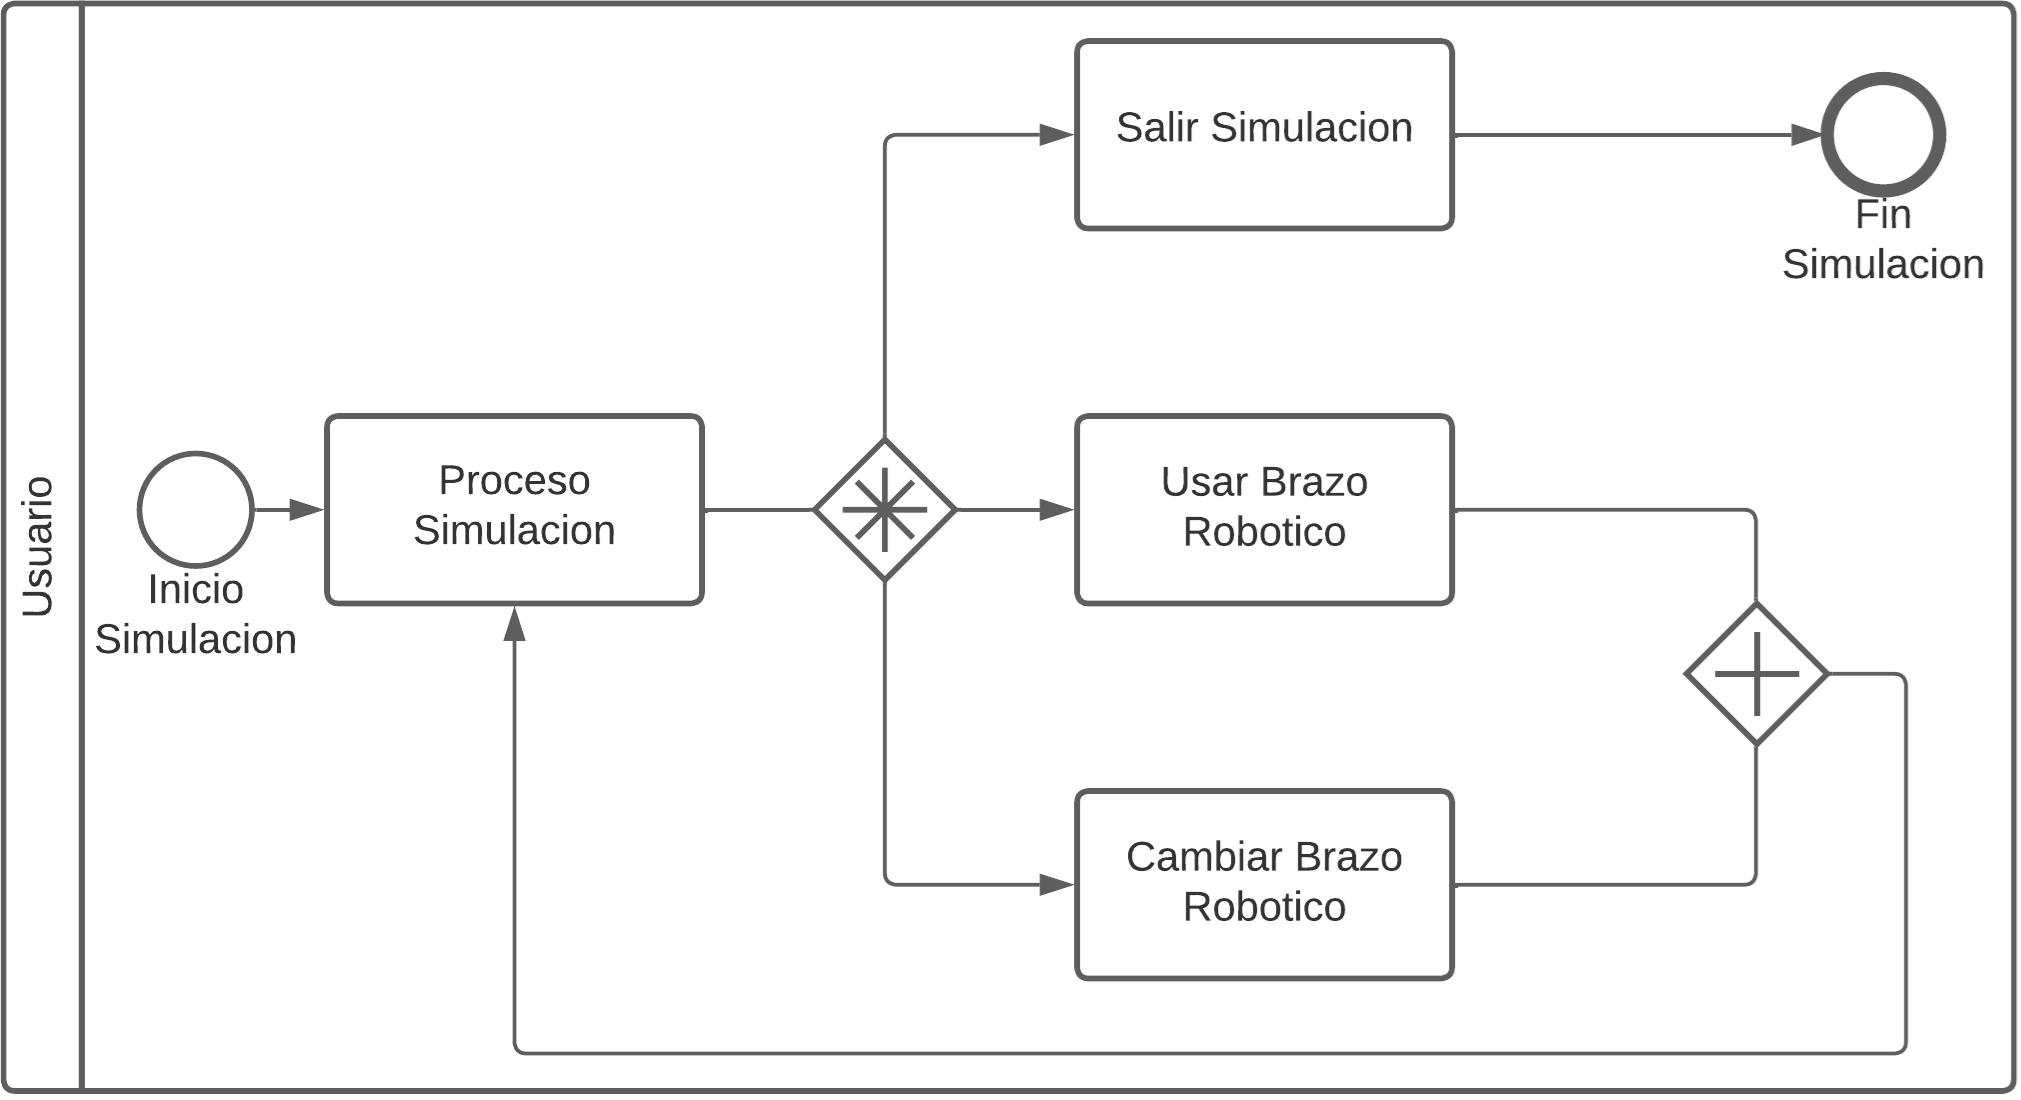
\includegraphics[height=6.83cm]{figures/bpmn.png}
\caption{Modelo y Notación de Procesos de Negocio}
\label{fig:bpmn}
\end{figure}

En la Figura 7.1 se muestra el proceso de como el usuario interactúa con la simulación, el proceso inicia con el usuario ejecutando la simulación, una vez dentro de esta, el usuario puede elegir entre usar el brazo robótico, cambiar de brazo robótico, con las cuales lo lleva a mantenerse en el proceso de la simulación, por ultimo esta la opción de salir de la simulación que finaliza este proceso

\section{Casos de uso}
\subsection{Actores}
Usuario: Persona que utilizara la aplicación, ya sea estudiante o profesor de la Universidad del Bío-Bío, como también personas externas a esta. El usuario puede utilizar la aplicación completamente.
\subsection{Diagrama de casos de uso y descripción}

\begin{figure}[h]
\centering
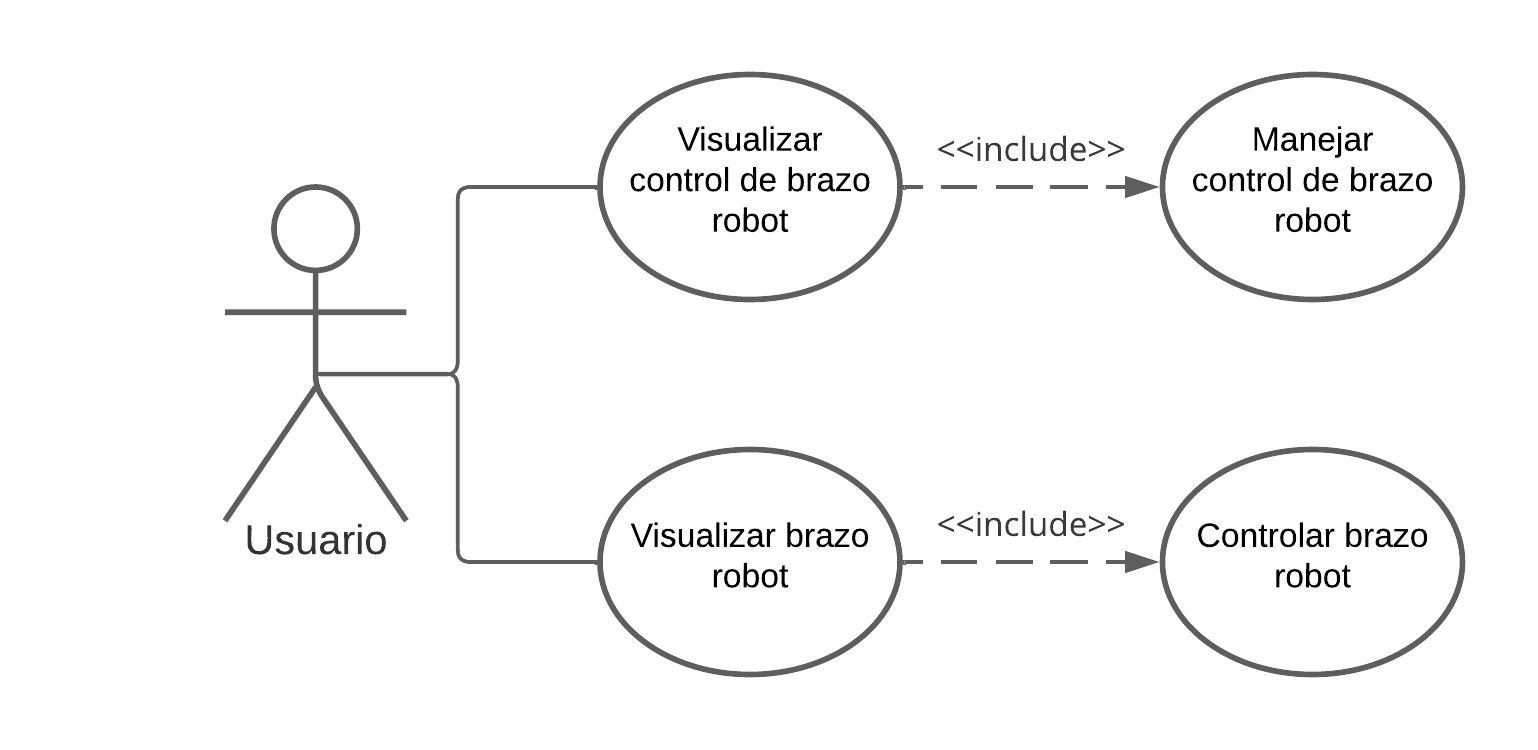
\includegraphics[height=6.83cm]{figures/usuario.png}
\caption{Diagrama de caso de uso: Usuario}
\label{fig:usuario}
\end{figure}

Como se logra apreciar en la Figura ~\ref{fig:usuario}, se muestran las interacciones que tiene el usuario en la aplicación. El actor es simplemente un usuario, ya que la aplicación es de uso personal.

\subsection{Especificación de los caso de uso}

\begin{table}[h!]
\begin{center}
\begin{tabular}{| m{0.19\linewidth} | m{0.75\linewidth} |}
\hline
\multicolumn{2}{ |c| }{Caso de Uso: Visualizar control de brazo robot} \\ \hline
ID & CU-01 \\ \hline
Descripción & El actor puede visualizar el control de brazo robot. \\ \hline
Actores & Usuario \\ \hline
Flujo principal & 

\begin{enumerate}[label=\arabic*.-]
    \item El actor debe haberse dirigido al menú desplegable
    \item El actor debe seleccionar la opción de "Visualizar Control"
\end{enumerate}

\\ \hline
\end{tabular}
\caption{Especificación de casos de uso: Visualizar control de brazo robot}
\end{center}
\end{table}

\begin{table}[h!]
\begin{center}
\begin{tabular}{| m{0.19\linewidth} | m{0.75\linewidth} |}
\hline
\multicolumn{2}{ |c| }{Caso de Uso: Manejar control de brazo robot} \\ \hline
ID & CU-02 \\ \hline
Descripción & El actor puede manejar el control de brazo robot. \\ \hline
Actores & Usuario \\ \hline
Flujo principal & 

\begin{enumerate}[label=\arabic*.-]
    \item El actor debe haberse dirigido al menú desplegable
    \item El actor debe seleccionar la opción de "Visualizar control de brazo robot"
\end{enumerate}

\\ \hline
\end{tabular}
\caption{Especificación de casos de uso: Manejar control de brazo robot}
\end{center}
\end{table}

\begin{table}[h!]
\begin{center}
\begin{tabular}{| m{0.19\linewidth} | m{0.75\linewidth} |}
\hline
\multicolumn{2}{ |c| }{Caso de Uso: Visualizar brazo robot} \\ \hline
ID & CU-03 \\ \hline
Descripción & El actor puede visualizar el brazo robot. \\ \hline
Actores & Usuario \\ \hline
Flujo principal & 

\begin{enumerate}[label=\arabic*.-]
    \item El actor debe haber abierto la aplicación
\end{enumerate}

\\ \hline
\end{tabular}
\caption{Especificación de casos de uso: Visualizar brazo robot}
\end{center}
\end{table}

\begin{table}[h!]
\begin{center}
\begin{tabular}{| m{0.19\linewidth} | m{0.75\linewidth} |}
\hline
\multicolumn{2}{ |c| }{Caso de Uso: Controlar brazo robot} \\ \hline
ID & CU-04 \\ \hline
Descripción & El actor puede controlar el brazo robot. \\ \hline
Actores & Usuario \\ \hline
Flujo principal & 

\begin{enumerate}[label=\arabic*.-]
    \item El actor debe haberse dirigido al menú desplegable
    \item El actor debe seleccionar el robot a utilizar
    \item El actor controla a través de teclado el robot
\end{enumerate}

\\ \hline
\end{tabular}
\caption{Especificación de casos de uso: Controlar brazo robot}
\end{center}
\end{table}